\subsection{Validation makes the diagnostic resolution explicit}
\label{sec:supportcontrols}
Controlled deletions verify which deficits the audit resolves. Removing one
joint Gaussian component while retaining all marginal modes is detected
in 200/200 trials at 1,000 samples per set. NDB also detects every joint
removal, while both projected rules detect 0/200. Combined removal,
contraction, and translation produce all three labels in 200/200 trials.
Rotation yields support departure in 198/200 trials with no expansion.

On cached image features, removing a 4.19\%-mass region is detected in
0/200, 196/200, and 200/200 trials at 250, 1,000, and 4,000 samples per set.
The smallest Gaussian null yields 4/200 expansion flags from the
approximate spread interval (Supp.~Sec.~C).

\begin{figure}[t]
\centering
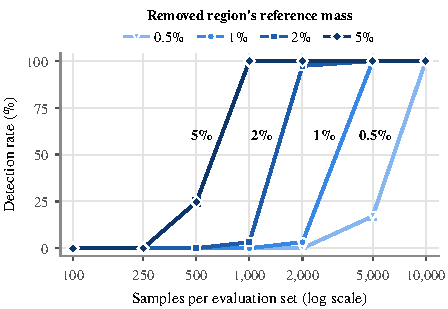
\includegraphics[width=\linewidth]{../figures/support_power_main.pdf}
\caption{Regional certificates have measurable resolution.
Complete removal, $M=10$, $\rho=0.5$, $\alpha_{\rm occ}=0.025$,
and eligibility 0.001 (distinct from the default 0.01).
Each point is 2,000 recorded trials with its saved exact 95\% binomial interval;
secondary analysis at the full-audit error level.}
\label{fig:support-main-power}
\end{figure}

Rare regions require more samples. In the power experiment with eligibility
0.001, detection for a 1\%-mass region rises
from 3.25\% at $n=2{,}000$ to 99.9\% at $n=5{,}000$
(Fig.~\ref{fig:support-main-power}); increasing the family from 10 to 440
reduces the latter to 73.95\%. With ten regions, 5,000 samples per set,
and a true ratio of 0.5, NDB flags a change in 83.4\% of trials.
The depletion test certifies a ratio below 0.5 in zero trials
(Supp.~Sec.~C.5). Equality testing can therefore flag a regional
change at sample sizes where an effect-size certificate remains unresolved.
The choice depends on whether the decision requires evidence of any change
or a lower bound on its magnitude.
